\section{Introduction}
The Kobuki is an educational ``turtle-bot" designed with hardware robustness and long lasting battery life to supply power to external devices. This allows us to connect the Kobuki up to a \texttt{NI myRIO-1900} reconfigurable I/O device and use the FPGA for implementing designs of a finite state machine (FSM) that navigates the Kobui through a 3x5m obstacle course. The arrangement of the myRIO on the Kobuki is shown in the Figure \ref{fig:kobuki}. The legend to the bottom right corner of Figure \ref{fig:kobuki} shows the orientation of the accelerometer ADXL330 used in myRIO. The forward direction for the Kobuki is the positive $x$ axis. 
\begin{figure}[H]
    \centering
    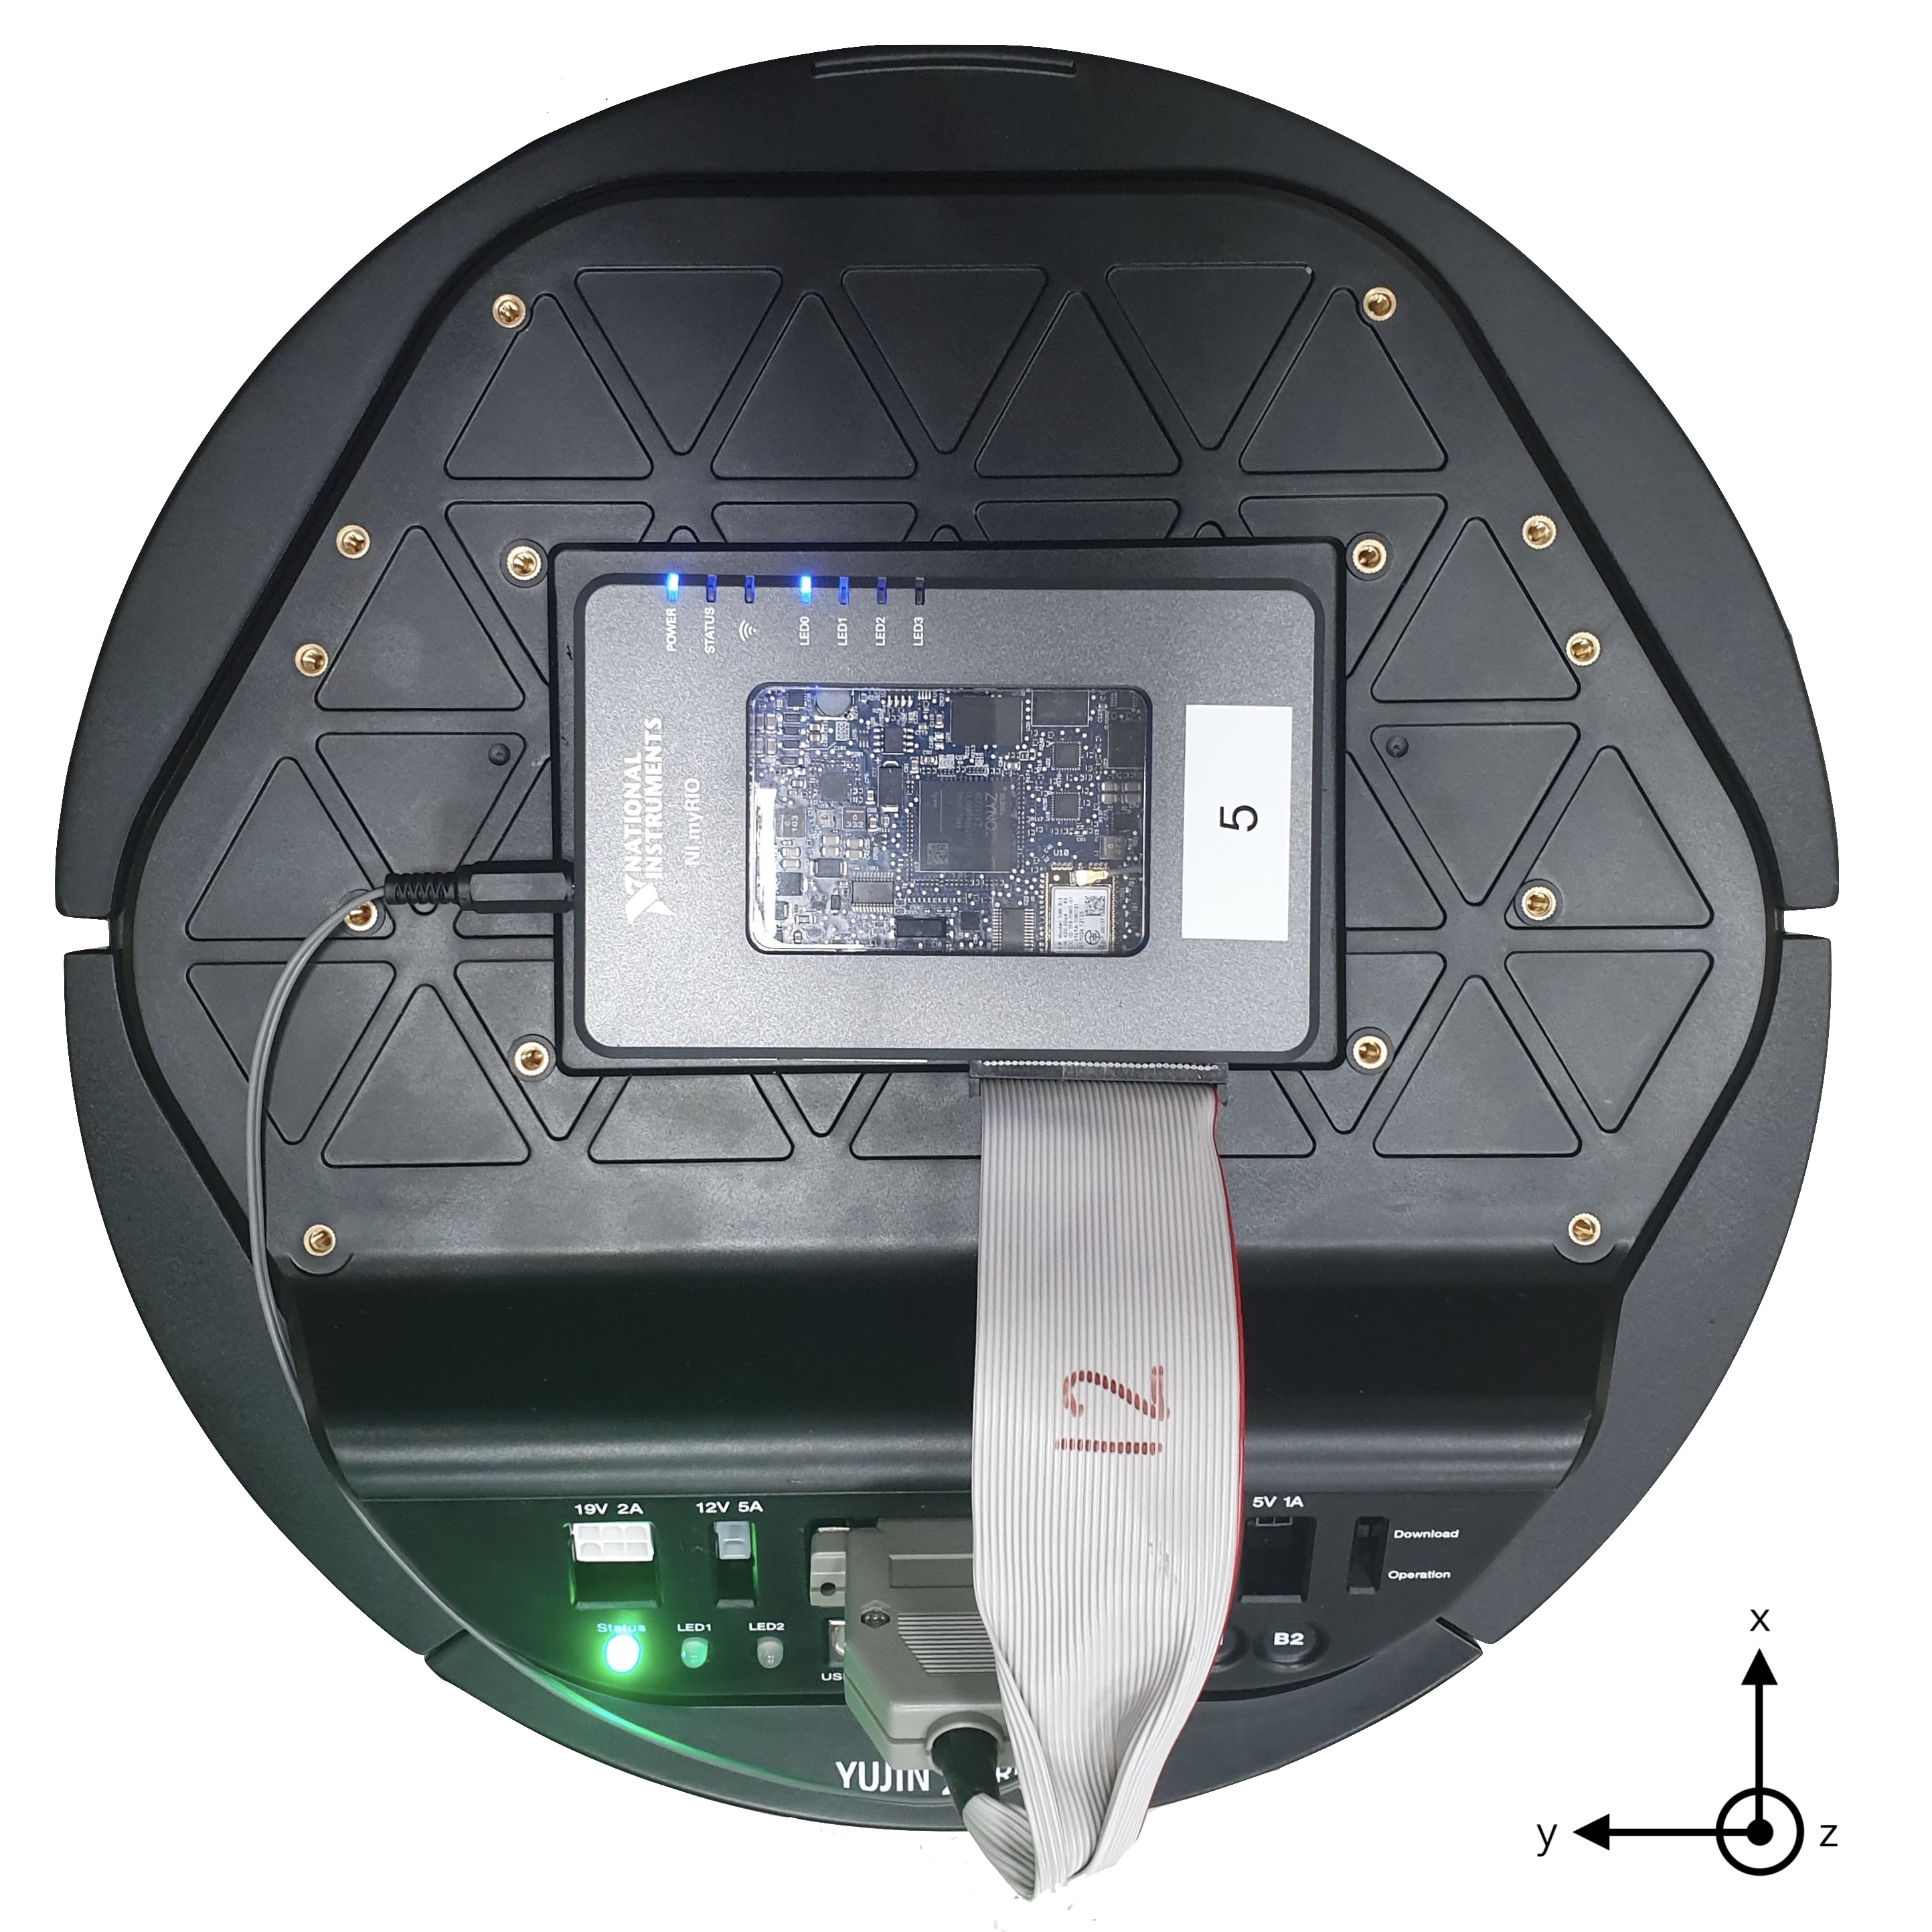
\includegraphics[width=8cm]{Images/Kobuki.png}
    \caption{30cm diameter Kobuki with connected myRIO in bird's eye view}
    \label{fig:kobuki}
\end{figure}

\subsection{Project Requirements}\label{sec:requirements}
To successfully complete the obstacle course, we must follow the following requirements and rules:
\begin{itemize}
    \item \textbf{Play/Pause}: 
    The Kobuki's action will be determined by it's 'B0' button. The robot shall only start when B0 is pressed. When pressed again all movement should be paused and the robot will resume upon another press of B0. The B0 button can also be referred to as the 'Play' button.
    \item \textbf{Driving}:
    The robot should stay level on the ground whilst moving at all times. The original positive $x$ axis position of the Kobuki at the start of the obstacle course determines the 'Ground Orientation', which the Kobuki should always follow. The ground orientation can only change after a power cycle, reprogram or restart of the robot or its embedded controller. There are also additional challenges to overcome whilst driving:
    \begin{itemize}
        \item \textbf{Obstacle Avoidance}:
        The Kobuki should always avoid obstacles in the form of cliffs, wheel hazards, and objects whilst driving even during simultaneous or shortly successive encounters. After encountering obstacles, the Kobuki must be able to reorient and resume driving in ground orientation. The Kobuki is allowed to touch objects as long as it changes course immediately to avoid the obstacle. 
        \item \textbf{Hill Climb}:
        The Kobuki must be able to climb up a hill, drive through the plateau and descend to a final stop on flat ground within 40cm of the bottom of the hill. The robot must be able to orient itself on the hill to execute an orthogonal climb or descent. At any time the robot must not go over the edge of the hill.
    \end{itemize}
    \item \textbf{Performance Specfications}
    \begin{itemize}
        \item \textbf{Rotation}: The Kobuki should not rotate more than 180 degrees.
        \item \textbf{Chattering}: Chattering and erratic movement should not be exhibited.
        \item \textbf{Abnormal Termination}: With the exception of power or mechanical failure, the robot should not stop at any time.
        \item \textbf{Obstacle Hugging}: The Kobuki is not allowed to repeated encounter the same obstacle for navigation.
        \item \textbf{Timeliness}: The obstacle course should be completed within 180 seconds.
    \end{itemize}
\end{itemize}